\documentclass[11pt, openany]{article}
\usepackage{pstricks,pstricks-add,pst-math,pst-xkey}
\usepackage[frenchb]{babel}
%\usepackage{slashbox}
\usepackage{graphicx}
\usepackage{amsmath,amssymb,amstext}
%\usepackage{comment}
\usepackage[utf8]{inputenc}
\usepackage[OT1]{fontenc}
\usepackage{pgf,tikz}
\usepackage{pgfplots}
\usepackage{floatpag}
\usepgfmodule{shapes}
\usetikzlibrary{arrows,patterns}
\usepackage[ps]{skak}
\usepackage{chessboard}
\newcounter{moncompteur}
\newtheorem{q}[moncompteur]{ \textbf{Question}}{}
\newtheorem{prop}[moncompteur]{ \textbf{Proposition}}{}
\newtheorem{df}[moncompteur]{ \textbf{Définition}}{}
\newtheorem{rem}[moncompteur]{ \textbf{Remarque}}{}
\newtheorem{theo}[moncompteur]{ \textbf{Théorème}}{}
\newtheorem{conj}[moncompteur]{ \textbf{Conjecture}}{}
\newtheorem{cor}[moncompteur]{ \textbf{Corollaire}}{}
\newtheorem{lm}[moncompteur]{ \textbf{Lemme}}{}
%\newtheorem{nota}[moncompteur]{ \textbf{Notation}}{}
%\newtheorem{conv}[moncompteur]{ \textbf{Convention}}{}
\newtheorem{exa}[moncompteur]{ \textbf{Exemple}}{}
\newtheorem{ex}[moncompteur]{ \textbf{Exercice}}{}
%\newtheorem{app}[moncompteur]{ \textbf{Application}}{}
%\newtheorem{prog}[moncompteur]{ \textbf{Algorithme}}{}
%\newtheorem{hyp}[moncompteur]{ \textbf{Hypothèse}}{}
\newenvironment{dem}{\noindent\textbf{Preuve}\\}{\flushright$\blacksquare$\\}
\newcommand{\cg }{[\kern-0.15em [}
\newcommand{\cd}{]\kern-0.15em]}
\newcommand{\R}{\mathbb{R}}
\newcommand{\K}{\mathbb{K}}
\newcommand{\N}{\mathbb{N}}
\newcommand{\Z}{\mathbb{Z}}
\newcommand{\C}{\mathbb{C}}
\newcommand{\U}{\mathbb{U}}
\newcommand{\Q}{\mathbb{Q}}
\newcommand{\B}{\mathbb{B}}
\newcommand{\card}{\mathrm{card}}
\newcommand{\norm}[1]{\left\lVert#1\right\rVert}
\pgfplotsset{compat=1.8}
\newcommand{\La}{\mathcal{L}}
\newcommand{\Ne}{\mathcal{N}}
\newcommand{\D}{\mathcal{D}}
\newcommand{\Ss}{\textsc{safestay}}
\newcommand{\Sg}{\textsc{safego}}
\newcommand{\M}{\textsc{move}}
\newcommand{\E}{\mathcal{E}}
\newcommand{\V}{\mathcal V}
\setlength{\parindent}{0pt}




\begin{document}
\floatpagestyle{plain}
\renewcommand{\labelitemi}{$\bullet$}
\title{Le problème des $ n$ reines}
\date{}
\author{}
\maketitle
\section*{Position du problème}

On se place sur un échiquier de taille $n \times n$, sur lequel $n$ reines sont disposées. On dit qu'une reine est \emph{menacée} si elle se trouve sur la même ligne, colonne ou diagonale qu'une autre reine. On cherche à placer les $n$ reines de sorte qu'aucune reine ne soit menacée. 

On va chercher, en partant d'une situation initiale quelconque, à déplacer les reines de sorte à atteindre une position dans laquelle aucune d'elles n'est menacée. Pendant ces déplacements, on va permettre à chaque case de contenir un nombre quelconque de reines simultanément, et aussi d'être marquée par des signaux provenant d'un nombre quelconque de directions, qui traduisent la présence d'une reine dans la direction d'où ils proviennent.

%Notons donc $\B$ l'ensemble $\{vrai, faux\}$ des booléens. 
%On associe à chaque case de coordonnées $(i,j)$ un état $x_{i,j} \in \B^8\times\N$. Les huit booléens correspondent à la présence ou à l'absence, en provenance de chacune des huit directions, d'un signal traduisant la présence d'une reine dans cette direction, et l'entier (compris entre $0$ et $n$) correspond au nombre de reines présentes sur la case.

%On dit qu'une case est \emph{sûre} si elle ne contient pas de signal ni de reine (état $(faux, faux, ..., faux, 0)$) et on entend par là que c'est une bonne case de destination pour une reine. Dans le cas contraire, la case est dite \emph{dangereuse}.

On cherche à se donner une procédure de mise à jour locale telle qu'à chaque pas de temps, les états de certaines cases sont modifiés à partir d'informations sur les cases voisines : création et transmission de signaux, déplacements de reines... L'objectif est que les signaux traduisent au mieux la présence ou l'absence de reines dans la direction d'où ils viennent, et que les reines menacées se déplacent au cours du temps pour chercher des cases sûres. On cherche également à ce que les reines ne bougent plus une fois qu'une solution est atteinte. 

On s'astreint à ne déplacer les reines que d'au plus une case par pas de temps, de sorte que la règle de mise à jour puisse rester purement locale. On voudrait ne déplacer les reines que sur des cases sûres, mais c'est trop restrictif : il existe des positions qui ne sont pas solution du problème mais où toutes les reines sont entourées de cases menacées (cf. Figure 1). En revanche, permettre aux reines de se déplacer sur des cases dangereuses sans utiliser les informations locales dont elles disposent donne des mouvements trop aléatoires pour qu'on puisse espérer atteindre une solution en un temps raisonnable. On fixe donc une probabilité $\varepsilon \in [0,1]$, qui correspond à la probabilité pour une reine qui envisage un déplacement vers une case dangereuse de l'effectuer (alors qu'un déplacement vers une case sûre réussit toujours). En fixant $\varepsilon$ assez petit (de l'ordre de $0.01$ par exemple), on privilégie les déplacements vers des cases sûres tout en se donnant quand même la possibilité de sortir de situations bloquées.


\begin{figure}
\centering

\newgame
\fenboard{7q/6q1/5q2/4q3/3q4/2q5/1q6/q7 b - - 0 1}
\notationoff
\showboard
\caption{Les reines sont toutes menacées, mais aucun déplacement d'une case ne conduit à une case sûre.}
\end{figure}

%\section*{La procédure de mise à jour}
\section*{Formalisation}

\subsection*{Représentation du système}

\noindent
On représente l'échiquier par l'ensemble $\La = \cg 0, n-1\cd^2$. On pose $\mathcal{P} = \{0,1\}$ et $\D = \{NW,N,NE,W,E,SW,S,SE\}$ l'ensemble des huit directions. L'état d'une cellule étant déterminé par le nombre de reines présentes et la présence ou l'absence d'un signal en provenance de chaque direction, on note $\mathcal{Q} = {\mathcal{P}^8}\times\N$ l'ensemble des états. Une \emph{configuration} est un élément de $\E=\mathcal{Q}^\La$. Pour toute configuration $x$, et toute cellule $c \in \La$, on note $x_c = (s_{x, c}, n_{x, c})$ l'état de la cellule $c$ dans la configuration $x$. 

\noindent
$n_{x,c}$ est le nombre de reines sur la cellule $c$ dans la configuration $x$, et $s_{x,c} = (s_{x,c,N}, s_{x,c,NE}, s_{x,c,E}, \ldots, s_{x,c,NW})$ code la présence ou l'absence de signaux venant de chaque direction : $s_{x,c,d}$ vaut $1$ si dans la configuration $x$, la cellule $c$ contient un signal provenant de la direction $d$, et $0$ sinon.


Par souci de lisibilité, on omettra les indices $x$ de configuration partout où on pourra le faire sans ambiguïté et on parlera de l'état $(s_c, n_c)$ d'une cellule $c$.
%La fonction $s_{x, c}$ associe à chaque direction $1$ si $c$ contient un signal en provenance de cette direction et $0$ sinon, et $c$ contient $n_{x, c}$ reines.

On pose $\Ne \subset \La^2$ l'ensemble des paires de cellules adjacentes : $$(c, c') \in \Ne \iff \norm{(c-c')}_\infty = 1$$

À chaque pas de temps, on choisit au hasard une paire de cases adjacentes et on les met à jour l'une par rapport à l'autre.
On se donne donc $(u_t)_{t\in\N} \in \Ne^\N$ la suite des paires de cellules mises à jour : pour tout $t\in\N$, la paire de cellules mises à jour à l'étape $t$ est $u_t$. Ce sont les valeurs d'une suite de variables aléatoires indépendantes à distribution uniforme sur $\Ne$. On définit de même $(x_t)_{t\in\N}$ la suite des configurations prises par le système au cours du temps. Initialement, aucun signal n'est présent et les $n$ reines sont réparties aléatoirement sur l'échiquier, selon une loi uniforme (de façon indépendante : notamment plusieurs reines peuvent se trouver initialement sur la même case). 

On cherche à définir une fonction de mise à jour globale $\mathcal{F} : {\E\times\Ne}\to\E$ qui à une configuration associe une configuration aléatoire qui lui succède selon la procédure de la partie précédente : $\mathcal{F}(x_t, u_t) = x_{t+1}$.

%Initialement, aucun signal n'est présent.
% et les $n$ reines sont réparties aléatoirement sur l'échiquier, selon une loi uniforme (de façon indépendante : notamment plusieurs reines peuvent se trouver initialement sur la même case). 
 
\subsection*{Choix des cases à mettre à jour}

On souhaite choisir une paire de cases adjacentes à mettre à jour, avec la même probabilité de choisir chaque paire de cases. On observe qu'il y a $n(n-1)$ paires de cases voisines verticalement, $n(n-1)$ horizontalement et $(n-1)^2$ selon chaque diagonale, soit $(4n-2)(n-1)$ paires de cases adjacentes au total. On applique donc la procédure de sélection suivante : \begin{itemize}

\item{On choisit selon une loi uniforme $N \in \cg 0, (4n-2)(n-1) -1 \cd$, on en déduit $A \in \cg 0, 4n-3 \cd$ et $B \in \cg 0, n-2\cd$ le quotient et le reste de la division euclidienne de $N$ par $(n-1)$.  }
\item{Si $A<n$, on prend les cases $(B,A)$ et $(B+1,A)$.}
\item{Si $A = n+i, i<n$ on prend les cases $(i,B)$ et $(i,B+1)$.}
\item{Si $A = 2n+i,i<n-1$ on prend $(i,B)$ et $(i+1, B+1)$.}
\item{Sinon, $A = 3n-1+i$ et $i<n-1$, et on prend $(i, B+1)$ et $(i+1, B)$.}
%\item{On choisit selon une loi uniforme une direction (parmi N, NW, NE, W, E, SW, SE, S)}.

%\item{On choisit selon une loi uniforme une case possédant une case voisine dans cette direction (c'est-à-dire ne se trouvant pas sur le mauvais bord de l'échiquier).}

%\item{Les cases à mettre à jour sont la case tirée au sort et sa voisine dans la direction tirée au sort.}

\end{itemize}
La fonction qui à $N$ associe une paire de cases adjacentes étant bijective, on a bien la même probabilité de choisir chaque paire de cases. 


\subsection*{Mise à jour : les déplacements}

On se donne deux cases adjacentes $c$ et $c'$ à mettre à jour. On commence par envisager des déplacements de reine entre $c$ et $c'$. Le principe général est qu'une reine menacée essaie de quitter sa case lorsqu'elle est mise à jour. Ce déplacement réussit ou non en fonction de l'état de l'autre case mise à jour, avec une part d'aléatoire. La procédure est la suivante :

\begin{itemize}

\item{ Si une reine est présente en case $c$, alors que la case $c$ contient un signal, elle essaie de se déplacer vers la case $c'$. De même, si plusieurs reines sont présentes en $c$, elles sont menacées et l'une d'entre elles tente de se déplacer vers la case $c'$.}

\item{ S'il n'y a pas de signal en $c'$ sauf éventuellement un venant de $c$ (qui est peut-être dû à la présence de la reine qui cherche à bouger), et qu'il n'y a pas d'autre reine en $c'$, la case est considérée comme sûre et le déplacement a lieu (cf. Figure $2$). Sinon, la case est dangereuse, et le déplacement a lieu seulement avec une probabilité $\varepsilon$.
% Si le déplacement réussit, on retire une reine à la case $c$ et on en ajoute une à la case $(i', j')$. 
}

\item{ Symétriquement, une reine de $c'$ peut se déplacer vers $c$ selon la même procédure. Les deux déplacements se font de manière simultanée afin que l'ordre des deux cases choisies pour la mise à jour n'ait pas d'importance.}

\end{itemize}
\medskip
Formalisons cette procédure à l'aide de quelques fonctions auxiliaires :  

 \begin{itemize}
  \item{On pose $\Ss : {\La}\to\{0,1\}$ qui indique si une reine peut rester sur une case donnée : \[
 \Ss(c) =
  \begin{cases} 
      \hfill 1    \hfill & \text{ si $n_c\leq 1$ et $\forall d \in \D, s_c(d)=0$} \\
      \hfill 0 \hfill & \text{ sinon} \\
  \end{cases}
\]}
 
  \item{On pose $\Sg :  {\La\times\D}\to\{0,1\}$ qui indique si une reine peut se déplacer de façon sûre vers une certaine case en venant d'une certaine direction : \[
 \Sg(c, d_{\mathrm {from}}) =
  \begin{cases} 
      \hfill 1    \hfill & \text{ si $n_c=0$ et $\forall d \in \D\setminus\{d_{\mathrm{from}}\}, s_c(d)=0$} \\
      \hfill 0 \hfill & \text{ sinon} \\
  \end{cases}
\]
 En toute rigueur, $\Ss$ et $\Sg$ devraient prendre aussi la configuration en argument : on l'omet pour plus de lisibilité.
}
\medskip
  \item{On pose $\delta :\Ne\to\D$ telle que $\delta(c_{\mathrm{from}}, c_{\mathrm{to}})$ soit la direction de $c_{\mathrm{from}}$ vue de $c_{\mathrm{to}}$. Plus formellement : \[
 \delta(c_{\mathrm{from}}, c_{\mathrm{to}}) =
  \begin{cases} 
    \hfill N    \hfill & \text{ si $c_{\mathrm{to}}-c_{\mathrm{from}}=(0,1)$} \\
    \hfill NE \hfill & \text{ si  $c_{\mathrm{to}}-c_{\mathrm{from}}=(1,1)$} \\
    \hfill \cdots & \\
    \hfill W \hfill & \text{ si  $c_{\mathrm{to}}-c_{\mathrm{from}}= (-1,0)$}\\
    \hfill NW \hfill & \text { si  $c_{\mathrm{to}}-c_{\mathrm{from}}=(-1,1)$}\\
  \end{cases}
\] }
  \item{On peut alors définir $\M :{\Ne}\to\{0,1\}$ qui traduit la procédure décrite ci-dessus : $\M(c_{\mathrm{from}}, c_{\mathrm{to}})$ vaut $1$ si une reine se déplace de $c_{\mathrm{from}}$ à $c_{\mathrm{to}}$ et $0$ sinon. Formellement : \[
    \M(c_{\mathrm{from}}, c_{\mathrm{to}}) = 
    \begin{cases}
      \hfill 0 \hfill & \text{ si $\Ss(c_{\mathrm{from}})=1$} \\
      \hfill 1 \hfill & \text{ si : }{ \begin{cases} \Ss(c_{\mathrm{from}})=0 \\\text{et $n_{c_{\mathrm{from}}}\geq 1$} \\ \text{et } \Sg(c_{\mathrm{to}}, \delta(c_{\mathrm{from}}, c_{\mathrm{to}}))=1\\ \end{cases}}\\

      \hfill \mathcal{B}(\varepsilon)\hfill  & \text{ sinon} \\
    \end{cases}
\]
où $\mathcal{B}(\varepsilon)$ est une variable aléatoire valant $1$ avec une probabilité $\varepsilon$ et $0$ avec une probabilité $1-\varepsilon$. Comme précédemment, on omet de passer la configuration en argument à $\M$ tant qu'il n'y a pas d'ambiguïté.
}


\end{itemize}

\medskip

On peut maintenant écrire $\mathcal{F}_{\mathrm{move}} : \E\times\Ne\to\E$ qui modifie la configuration par d'éventuels déplacements de reine entre les cases mises à jour :  \[
\mathcal{F}_{\mathrm{move}}(x,(c_1, c_2)) = 
\begin{cases}
  \hfill x_{c_1\to c_2} \hfill & \text{ si $\M(c_1, c_2) = 1$ et $\M(c_2, c_1) = 0$} \\
  \hfill x_{c_2 \to c_1} \hfill & \text{ si $\M(c_1, c_2) = 0$ et $\M(c_2, c_1) = 1$} \\
  \hfill x \hfill & \text{ sinon} \\
  \end{cases}
\]
où $x_{a \to b}$ désigne la configuration obtenue à partir de $x$ en retranchant $1$ à $n_{a}$ et en ajoutant $1$ à $n_{b}$. 

\medskip



\subsection*{Mise à jour : les signaux}  

Après avoir effectué d'éventuels déplacements de reine, on met à jour les signaux de $c$ et $c'$. 

 \begin{itemize} 

\item{% Le signal en $c'$ provenant de la direction de $c$ est modifié de la façon suivante : il devient vrai 
Un signal en $c'$ provenant de la direction de $c$ apparaît ou reste présent s'il y a une reine en $c$, (cf. Figure $2$) ou s'il y a un signal en $c$ dans la même direction (intuitivement, il y a une reine plus loin dans la direction de $c$) (cf. Figure $3$). Sinon, rien n'indique plus la présence d'une reine dans cette direction : le signal disparaît s'il était présent (cf. Figure $4$). }

\item{ Symétriquement, le signal en $c$ provenant de $c'$ est mis à jour de la même façon.}

\item{ Les autres signaux ne sont pas modifiés. }
  
%Le booléen de $x_{i,j}$ correspondant à la direction $d_{2\rightarrow 1}$ devient vrai s'il y a au moins une reine sur la case $c'$ ou si le booléen de $x_{i',j'}$ correspondant à  $d_{2\rightarrow 1}$  est vrai (intuitivement, il y a alors une reine plus loin dans cette direction), et devient faux sinon.

% Symétriquement, le booléen de $x_{i', j'}$ correspondant à $d_{1\rightarrow 2}$ devient vrai s'il y a une reine en $c$ ou si le booléen de $x_{i,j}$ correspondant à $d_{1\rightarrow 2}$ est vrai, et devient faux dans le cas contraire.}

\end{itemize}

\bigskip

\noindent 
Formellement, on pose, pour tout %$x\in\E$, $(c,c')\in\Ne$, 
$d\in\D$, le signal mis à jour $s_{x, c, d}^{c'}$ :  \[
s_{x, c, d}^{c'} = 
\begin{cases}
  \hfill s_{x, c, d} \hfill & \text{ si $d \neq \delta(c', c)$} \\
  \hfill 1 \hfill & \text{ si $d = \delta(c', c)$ et $n_{x, c'}\geq 1$} \\
  \hfill s_{x, c', d} \hfill & \text{ sinon}\\
\end{cases}
\]

$s_{x, c, d}^{c'}$ est le signal de la case $c$ se rapportant à la direction $d$, et mis à jour par rapport à la case $c'$. On va s'en servir pour définir une fonction $\mathcal{F}_{\mathrm{sign}} : \E\times\Ne\to\E$ de mise à jour des signaux :
\noindent
 $\mathcal{F}_{\mathrm{sign}} (x, (c_1, c_2)) = x'$ avec : \[
\begin{cases}
  \hfill x'_{c_1} = (s_{x, c_1}^{c_2}, n_{x,c_1}) \hfill & \\
  \hfill x'_{c_2} = (s_{x, c_2}^{c_1}, n_{x, c_2}) \hfill & \\
  \hfill x'_c = x_c  \hfill & \text{pour tout $c \notin \{ c_1, c_2\}$} \\
\end{cases}
\]

\bigskip

\noindent
On peut alors définir la fonction de mise à jour : $$\mathcal{F}(x_t, u_t) = \mathcal{F}_{\mathrm{sign}}(\mathcal{F}_{\mathrm{move}}(x_t, u_t), u_t)$$


On remarque que lors de la mise à jour d'une case, la nouvelle valeur du signal qu'on modifie ne dépend pas de l'ancienne valeur, mais seulement de la case voisine : les signaux sont transmis localement de manière instantanée mais les cases n'ont pas de mémoire. Ainsi, lorsqu'une reine quitte une rangée de cases, les signaux dans cette direction n'arrivent plus et l'information de l'absence de cette reine est propagée. 

L'asynchronisme de la mise à jour est utile : si on mettait les cases à jour de façon synchrone, deux reines sur la même ligne, colonne ou diagonale recevraient en même temps l'information, et pourraient se déplacer toutes les deux en même temps alors que le comportement souhaité est qu'une seule des deux reines se déplace. 


 \definecolor{ffqqqq}{rgb}{1,0,0}
\definecolor{xdxdff}{rgb}{0.49,0.49,1}
\definecolor{zzttqq}{rgb}{0.6,0.2,0}
\definecolor{uququq}{rgb}{0.25,0.25,0.25}
\definecolor{qqqqff}{rgb}{0,0,1}


\begin{figure}[p]
\centering
\begin{tikzpicture}[line cap=round,line join=round,>=triangle 45,x=1.0cm,y=1.0cm]
\clip(-8.56,-0.74) rectangle (4.7,2.48);
%\fill[color=zzttqq,fill=zzttqq,fill opacity=0.1] (0,2) -- (0,0) -- (2,0) -- (2,2) -- cycle;
%\fill[color=zzttqq,fill=zzttqq,fill opacity=0.1] (2,2) -- (2,0) -- (4,0) -- (4,2) -- cycle;
%\fill[color=zzttqq,fill=zzttqq,fill opacity=0.1] (-7.7,2) -- (-7.7,0) -- (-5.7,0) -- (-5.7,2) -- cycle;
%\fill[color=zzttqq,fill=zzttqq,fill opacity=0.1] (-5.7,2) -- (-5.7,0) -- (-3.7,0) -- (-3.7,2) -- cycle;
\draw [color=zzttqq] (0,2)-- (0,0);
\draw [color=zzttqq] (0,0)-- (2,0);
\draw [color=zzttqq] (2,0)-- (2,2);
\draw [color=zzttqq] (2,2)-- (0,2);
\draw [color=zzttqq] (2,2)-- (2,0);
\draw [color=zzttqq] (2,0)-- (4,0);
\draw [color=zzttqq] (4,0)-- (4,2);
\draw [color=zzttqq] (4,2)-- (2,2);
\draw [->] (2,1) -- (1.5,1);
\draw (1.02,-0.14) node[anchor=north west] {1};
\draw (2.94,-0.14) node[anchor=north west] {2};
\draw [color=zzttqq] (-7.7,2)-- (-7.7,0);
\draw [color=zzttqq] (-7.7,0)-- (-5.7,0);
\draw [color=zzttqq] (-5.7,0)-- (-5.7,2);
\draw [color=zzttqq] (-5.7,2)-- (-7.7,2);
\draw [color=zzttqq] (-5.7,2)-- (-5.7,0);
\draw [color=zzttqq] (-5.7,0)-- (-3.7,0);
\draw [color=zzttqq] (-3.7,0)-- (-3.7,2);
\draw [color=zzttqq] (-3.7,2)-- (-5.7,2);
\draw [->,dash pattern=on 1pt off 1pt] (-3.1,0.98) -- (-0.58,1);
\draw (-6.94,-0.22) node[anchor=north west] {1};
\draw (-4.66,-0.2) node[anchor=north west] {2};
\draw [->] (-6.7,2) -- (-6.7,1.5);
\draw [->] (1,2) -- (1,1.5);
\draw [fill=black,pattern=north east lines] (-6.74,0.96) circle (0.29cm);
\draw [fill=black,pattern=north east lines] (3.04,1.02) circle (0.29cm);
\end{tikzpicture}
%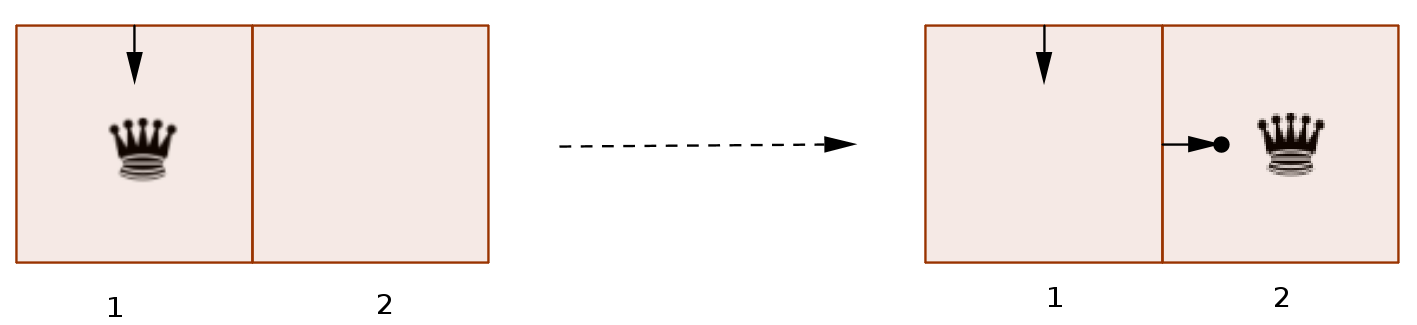
\includegraphics[scale=1.2]{schema2.png}
\caption{La reine présente en 1, menacée depuis le nord, se déplace en 2 qui est une case sûre, puis les signaux sont mis à jour : il y a une reine en 2, donc un signal venant de l'est apparaît en 1.}
\end{figure}
\begin{figure}[p]
\centering
\begin{tikzpicture}[line cap=round,line join=round,>=triangle 45,x=1.0cm,y=1.0cm]
\clip(-8.56,-0.74) rectangle (4.7,2.48);
%\fill[color=zzttqq,fill=zzttqq,fill opacity=0.1] (0,2) -- (0,0) -- (2,0) -- (2,2) -- cycle;
%\fill[color=zzttqq,fill=zzttqq,fill opacity=0.1] (2,2) -- (2,0) -- (4,0) -- (4,2) -- cycle;
%\fill[color=zzttqq,fill=zzttqq,fill opacity=0.1] (-7.7,2) -- (-7.7,0) -- (-5.7,0) -- (-5.7,2) -- cycle;
%\fill[color=zzttqq,fill=zzttqq,fill opacity=0.1] (-5.7,2) -- (-5.7,0) -- (-3.7,0) -- (-3.7,2) -- cycle;
\draw [color=zzttqq] (0,2)-- (0,0);
\draw [color=zzttqq] (0,0)-- (2,0);
\draw [color=zzttqq] (2,0)-- (2,2);
\draw [color=zzttqq] (2,2)-- (0,2);
\draw [color=zzttqq] (2,2)-- (2,0);
\draw [color=zzttqq] (2,0)-- (4,0);
\draw [color=zzttqq] (4,0)-- (4,2);
\draw [color=zzttqq] (4,2)-- (2,2);
\draw [->] (0,2) -- (0.5,1.48);
\draw [->] (0,1) -- (0.5,1);
\draw [->] (2,1) -- (2.5,1);
\draw (1.02,-0.14) node[anchor=north west] {1};
\draw (2.94,-0.14) node[anchor=north west] {2};
\draw [color=zzttqq] (-7.7,2)-- (-7.7,0);
\draw [color=zzttqq] (-7.7,0)-- (-5.7,0);
\draw [color=zzttqq] (-5.7,0)-- (-5.7,2);
\draw [color=zzttqq] (-5.7,2)-- (-7.7,2);
\draw [color=zzttqq] (-5.7,2)-- (-5.7,0);
\draw [color=zzttqq] (-5.7,0)-- (-3.7,0);
\draw [color=zzttqq] (-3.7,0)-- (-3.7,2);
\draw [color=zzttqq] (-3.7,2)-- (-5.7,2);
\draw [->] (-7.7,2) -- (-7.2,1.5);
\draw [->] (-7.7,1) -- (-7.2,1);
\draw [->,dash pattern=on 1pt off 1pt] (-3.1,0.98) -- (-0.58,1);
\draw (-6.94,-0.22) node[anchor=north west] {1};
\draw (-4.66,-0.2) node[anchor=north west] {2};

\end{tikzpicture}
\caption { Le signal de la cellule 1 venant de l'ouest est transmis à la cellule 2.}
\end{figure}

\begin{figure}[p]
\centering
\definecolor{zzttqq}{rgb}{0.6,0.2,0}
\begin{tikzpicture}[line cap=round,line join=round,>=triangle 45,x=1.0cm,y=1.0cm]
\clip(-8.56,-0.74) rectangle (4.7,2.48);
\draw [color=zzttqq] (0,2)-- (0,0);
\draw [color=zzttqq] (0,0)-- (2,0);
\draw [color=zzttqq] (2,0)-- (2,2);
\draw [color=zzttqq] (2,2)-- (0,2);
\draw [color=zzttqq] (2,2)-- (2,0);
\draw [color=zzttqq] (2,0)-- (4,0);
\draw [color=zzttqq] (4,0)-- (4,2);
\draw [color=zzttqq] (4,2)-- (2,2);
\draw (1.02,-0.14) node[anchor=north west] {1};
\draw (2.94,-0.14) node[anchor=north west] {2};
\draw [color=zzttqq] (-7.72,2)-- (-7.72,0);
\draw [color=zzttqq] (-7.72,0)-- (-5.72,0);
\draw [color=zzttqq] (-5.72,0)-- (-5.72,2);
\draw [color=zzttqq] (-5.72,2)-- (-7.72,2);
\draw [color=zzttqq] (-5.72,2)-- (-5.72,0);
\draw [color=zzttqq] (-5.72,0)-- (-3.72,0);
\draw [color=zzttqq] (-3.72,0)-- (-3.72,2);
\draw [color=zzttqq] (-3.72,2)-- (-5.72,2);
\draw [->,dash pattern=on 1pt off 1pt] (-3.1,0.98) -- (-0.58,1);
\draw (-6.94,-0.22) node[anchor=north west] {1};
\draw (-4.66,-0.2) node[anchor=north west] {2};
\draw [->] (-6.72,0) -- (-6.72,0.5);
\draw [->] (1,0) -- (1,0.5);
\draw [->] (-5.72,1) -- (-6.22,1);
\end{tikzpicture}
\caption{Le signal en 1 venant de l'est disparaît.}
\end{figure}

\clearpage




\section*{Quelques observations expérimentales}


Lancé à partir d'une situation de départ aléatoire (la case de départ de chacune des $n$ reines est choisie selon une loi uniforme de façon indépendante), on observe que le système finit par atteindre un point fixe où chaque reine est sur une case sans signal. La position des reines est alors solution du problème des $n$ reines.

\subsection*{Comportement qualitatif}

On observe en général un régime transitoire sur les premiers milliers de pas de temps, pendant lesquels les signaux ne se sont pas encore propagés sur tout l'échiquier, donc pendant lesquels les mouvements des reines sont trop libres par rapport à la situation globale. Les mouvements des reines sont ensuite très restreints : une fois les signaux convenablement propagés, il y a très peu de cases sûres sur l'échiquier, voire aucune. De temps en temps, une reine se déplace vers une case dangereuse, ce qui libère certaines cases ; des déplacements vers des cases devenues sûres ont lieu puis on retrouve une situation de blocage, et ainsi de suite jusqu'à ce qu'une solution soit trouvée.

\subsection*{Effets de $\boldsymbol \varepsilon$}



Le paramètre $\varepsilon$ a des effets multiples. Plus $\varepsilon$ est grand, plus le système sort rapidement de situations bloquées où aucun déplacement vers une case sûre n'est possible. En revanche, plus il est petit, plus le système a tendance à effectuer tous les déplacements possibles vers des cases sûres avant de déplacer une reine vers une case dangereuse, ce qui peut empêcher de passer à côté d'une solution. En effet, si une solution est accessible sans avoir besoin de déplacer de reine vers une case dangereuse, plus $\varepsilon$ est grand, plus le risque de déplacer une reine vers une case dangereuse et d'avoir peu de chances de trouver rapidement cette solution est important. Enfin, comme il y a typiquement très peu de cases sûres, $\varepsilon$ contrôle également la fréquence des déplacements : plus il est petit, plus les signaux ont de temps pour se propager sur l'échiquier avant le prochain déplacement de reine. Ceci implique que plus $\varepsilon$ est petit, plus les reines se déplacent en se basant sur des informations à jour. 

Le choix de $\varepsilon$ pour minimiser le temps mis par le système pour trouver une solution relève donc d'un compromis entre ces différents effets : on le voudrait petit pour privilégier les déplacements sûrs et déplacer les reines à partir d'informations valides, mais grand pour que les déplacements soient suffisament fréquents.

La figure $5$ représente la variation du temps de convergence (le nombre de mises à jour avant d'atteindre une solution) et du nombre de déplacements effectifs de reine en fonction de la probabilité $\varepsilon$, dans le cas $n=8$. Les valeurs sont des moyennes sur $100$ échantillons, sauf les deux points extrémaux où l'on s'est restreint à $30$ échantillons pour des raisons de temps de calcul. On observe un optimum de $\varepsilon$ pour ce qui est du temps de convergence, autour de $0.01$, tandis que le nombre de déplacements croît avec $\varepsilon$ sur les valeurs considérées. 

La monotonie apparente du nombre de déplacements en fonction de $\varepsilon$ n'est pas étonnante : diminuer $\varepsilon$ revient à augmenter la qualité des déplace\-ments (plus souvent vers des cases sûres, avec des informations plus à jour) quitte à ce qu'ils aient lieu moins fréquemment.

%Un début d'explication à l'existence d'un optimum pour $\varepsilon$ est le fait que sa valeur est un compromis entre le besoin de sortir de situations bloquées (on a besoin de $\varepsilon$ grand) et celui de privilégier les cases sûres pour se diriger vers une solution (il faudrait $\varepsilon$ petit). En effet, plus $\varepsilon$ est grand, plus les reines ont tendance à se déplacer alors que les modifications récentes aux signaux n'ont pas été propagées, donc à se déplacer à partir d'informations erronées.

Ce modèle ne fait pas de distinction entre les cases dangereuses : on aurait pu envisager, par exemple, de toujours autoriser les déplacements vers des cases portant moins de signaux que la case de départ. Ceci autorise beaucoup de déplacements de reine et le comportement du système est analogue à celui de notre modèle avec $\varepsilon$ très élevé : la convergence, s'il y en a une, est en fait moins rapide. 

\subsection*{Temps de convergence en fonction de $\boldsymbol n$}

  

La figure $6$ représente l'évolution du temps de convergence en fonction de $n$, dans le cas $\varepsilon=0.01$. Le temps de convergence semble exponentiel en $n$. On a tracé sur la même figure la variation, en fonction de $n$, de $1/d$ où $d$ est la densité des solutions au problème des n reines (quotient du nombre de solutions par le nombre total de positions). Le nombre de solutions est une valeur tabulée par recherche exhaustive \footnote{http://jsomers.com/nqueen\_demo/nqueens.html}. On constate que $d$ décroît également exponentiellement, ce qui tend à expliquer la croissance rapide du temps de convergence. L'irrégularité au point $n=6$ s'explique de même par le fait que la variation du nombre de solutions au problème présente la même irrégularité. En effet, il existe $10$ solutions au problème pour $n=5$, mais seulement $4$ pour $n=6$ alors qu'asymptotiquement, le nombre de solutions croît exponentiellement, même si le nombre total de positions croît encore plus rapidement.

\begin{figure}
  \centering
  \begin{tikzpicture}
  \begin{axis}[%
      width=\textwidth,
      scaled y ticks=false,
      scaled x ticks=false,
      xtick = {0, 0.005, 0.01, 0.015, 0.02},
      xticklabel style={
        /pgf/number format/fixed,
        /pgf/number format/precision=5
      },
      xlabel=$\varepsilon$,
      ylabel=Temps de convergence,
      legend style={at={(0.25,-0.20)},
        anchor=north}]
    \addplot[color=red, mark = *] coordinates {%(0.0005, 4186672) 
(0.001, 1677950) 
      (0.005, 508333)%(0.008, 414684) 
      (0.01, 372401) 
      %(0.012, 418484)
      (0.015, 477431)  (0.02, 672129)    %(0.03, 1324725)
    }; 
    \addlegendentry{Temps de convergence}
        
  \end{axis}
  \begin{axis}[%
      width=\textwidth,
      hide x axis,
      axis x line=none,
      scaled x ticks=false,
      yticklabel style={
        /pgf/number format/fixed,
        /pgf/number format/precision=5,
        /pgf/number format/1000 sep={}
      },
      axis y line*=right,
      legend style={at={(0.75,-0.20)},anchor=north},
      xlabel near ticks,
      ylabel={Nombre de déplacements},
      ylabel near ticks]
    \addplot[color=blue, mark = triangle*] coordinates {% (0.0005, 499) 
(0.001, 403)
      (0.005, 641)
      %(0.008, 883)
      (0.01, 996)
      %(0.012, 1368)
      (0.015, 1997)(0.02, 3731)% (0.03, 10998)
    };
    \addlegendentry{Nombre de déplacements}
  \end{axis}
  \end{tikzpicture}
  \caption{Temps de convergence moyen et nombre moyen de déplacements en fonction de $\varepsilon$ pour $n=8$.}
\end{figure}   

\begin{figure}
  \thisfloatpagestyle{empty}
  \centering
  \begin{tikzpicture}
  \begin{axis}[%
      width=\textwidth,
      ymode=log,
      scaled y ticks=false,
      scaled x ticks=false,
      xlabel=$n$,
      ylabel={Temps de convergence}]
    \addplot[color=red, mark = *] coordinates {(4, 2730) (5, 6280)
      (6, 89530) (7, 110190) (8, 372401) (9, 865766) (10, 5005116) 
      (11, 14883900) 
      (12, 73200000)
    }; 
  \end{axis}
  \end{tikzpicture}

  \begin{tikzpicture}
  \begin{axis}[%
      width=\textwidth,
      ymode=log,
     %ticklabel style={
      %  /pgf/number format/fixed,
       % /pgf/number format/precision=5,
       % /pgf/number format/1000 sep={}
     % },
      xlabel=$n$,
      ylabel={$1/d$},
      ylabel near ticks]
    \addplot[color=blue, mark = triangle*] coordinates {
      (4, 32768) (5, 976562.5) (6, 544195584) (7, 16955576821) (8, 3.06e12) (9, 4.26e14) (10, 1.38e17) (11, 3.04e19) (12, 5.60e21)
 };
  \end{axis}
  \end{tikzpicture}
  \caption{Temps de convergence pour $\varepsilon=0.01$ et inverse de la densité de solutions en fonction de $n$  (échelle logarithmique).}
\end{figure} 


\section*{Un autre algorithme}

Le modèle précédent ne passe pas très bien à l'échelle : obtenir une solution pour des tailles supérieures à $12$ peut s'avérer très long. On va donc envisager un nouveau modèle dans lequel plus d'informations sont prises en compte à chaque étape de calcul. L'objectif est que l'évolution du système soit plus dirigée que précédemment, tout en se restreignant encore à des règles de mise à jour locales. Plutôt que de choisir une paire de cases à chaque pas de temps et ne considérer que les informations contenues dans ces deux cases, on va mettre à jour une case par pas de temps, en utilisant les informations de toutes ses voisines. 

On utilise le même système de signaux que dans l'algorithme précédent et on garde le même espace d'états : $\mathcal{Q} = {\mathcal{P}^8}\times\N$. On pose, pour tout $c\in\La$, $\V_c\subset\La$ l'ensemble des cellules voisines de $c$ : $\V_c = \{c' \in \La, \norm{(c-c')}_\infty = 1\}$.
À chaque pas de temps, on choisit une case au hasard, on met à jour ses signaux par rapport à ceux des cellules voisines, et une reine quitte éventuellement la case. 

%On se donne $(u_t)_{t\in\N} \in \La^\N$ la suite des cellules mises à jour, et $(x_t)$ la suite des configurations, et on va définir $\mathcal{F'} : \E\times\La\to\E$ telle que $\mathcal{F'}(x_t,u_t) = x_{t+1}$.

\bigskip

Contrairement à l'algorithme précédent, comme les signaux d'une seule case sont modifiés à chaque pas de temps, on les met à jour avant d'envisager un déplacement de reine. On met à jour les signaux d'une cellule $c$ par rapport à chacune de ses voisines, de la même façon que dans le modèle précédent : pour toute cellule $c'\in\V_c$, le signal en $c$ provenant de $c'$ apparaît ou reste présent s'il y en a un en $c'$ provenant de la même direction, ou s'il y a une reine en $c'$. Dans le cas contraire, il disparaît ou n'apparaît pas.
\bigskip

L'idée de la procédure pour déplacer une reine est la suivante : si on met à jour une case $c$ contenant des reines menacées, l'une d'entre elles choisit une case de $\V_c$, et tente de s'y déplacer selon la même procédure que dans l'algorithme précédent. 

On définit $\omega : \La\to\N\cup\{\infty\}$ qui sert à quantifier à quel point une cellule est dangereuse, de la façon suivante : \[
\omega(c) = 
\begin{cases}
  \hfill \infty \hfill \text{ si $n_c > 0$}\\
  \hfill \sum\limits_{d\in\D}s_{c,d} \hfill \text{ sinon}
\end{cases}
\]

On aimerait toujours envoyer une reine menacée de $c$ vers une cellule de $V_c$ qui minimise $\omega$, mais il existe des positions pour lesquelles un tel choix déterministe ne permet pas de résoudre le problème. Ainsi, la position de la figure $7$, avec les signaux convenablement propagés (ie. une case porte un signal venant d'une certaine direction si et seulement si il y a effectivement une reine dans cette direction), est une position insoluble. En effet, en partant de cette position, on aura à chaque instant les reines des colonnes \textbf c à \textbf f sur leur case initiale, et les deux autres dans le triangle de cases colorées en rouge, ce qui ne peut constituer une solution. 
Lorsqu'elles bougent, les deux reines du triangle rouge restent dedans : à chaque instant, la case rouge inoccupée vérifie $\omega = 2$, contre $3$ ou $4$ pour les cases adjacentes au triangle rouge. Quelque soit la position des deux reines dans le triangle rouge, les autres reines ne sont pas menacées : à chaque instant, le prochain mouvement est donc celui d'une des deux reines du triangle rouge, et elle reste dans ce triangle.


% TODO : figure

\begin{figure}[scale=0.85]
\centering
%\newchessgame
\chessboard[maxfield=f6,
  setpieces={qa3,qb3,qc6,qd4,qe1,qf5},pgf=true,captrimtoprint=true,psset=true, psskak=true,
color=red!50,
colorbackfields={a2,a3,b3}]

%\chessboard[maxfield=f6, setpieces={qa3,qb3,qc6,qd4,qe1,qf5}]
\caption{Exemple de position insoluble avec $\eta=0$.}
\end{figure}

\medskip

On veut donc que le choix de la destination ne soit pas toujours la case adhacente qui minimise $\omega$. On se donne donc une probabilité $\eta \in [0,1]$, et on choisit avec une probabilité $\eta$ une case aléatoire de $V_c$ comme destination, et avec une probabilité $1 - \eta$ une case aléatoire parmi les éléments de $V_c$ qui minimisent $\omega$. Ainsi, la position de la figure $7$ ne pose pas de problème pour $\eta > 0$ : une reine va sortir du triangle rouge et faire se déplacer une des autres reines.

Une fois la destination choisie, la procédure qui décide si le déplacement se fait ou non est exactement la fonction $\M$ de l'algorithme précédent.

\bigskip

\begin{figure}
  \centering
  \begin{tikzpicture}
  \begin{axis}[%
      width=\textwidth,
      ymode=log,
      scaled y ticks=false,
      scaled x ticks=false,
      xlabel={$n$},
      ylabel={Temps de convergence},
      legend entries = {Algorithme 1, Algorithme 2},
      legend style = {legend pos=north west}]
    \addplot[color=red, mark = *] coordinates {
      %(4, 2730) (5, 6280) (6, 89530) 
      (7, 110190) (8, 372401) (9, 865766) (10, 5005116) 
      (11, 14883900) 
      (12, 73200000)
    }; 
    \addplot[color=blue, mark = triangle*] coordinates {
      %(4, 837) (5, 1590) (6,2.78e4) 
      (7, 2.49e4) (8, 9.63e4) (9, 1.91e5) (10, 4.74e5) (11, 9.44e5) (12, 1.78e6)
    };
    %\addlegendentry{Temps de convergence}
        
  \end{axis}
  \end{tikzpicture}
  \caption{Temps de convergence moyen en fonction de $n$.}
\end{figure}  

La figure $8$ montre que ce nouvel algorithme passe un peu mieux à l'échelle que précédemment : la pente de la courbe qui représente le temps de convergence moyen en fonction de $n$ est plus basse pour le nouvel algorithme que pour l'ancien. De fait, il permet de trouver en un temps raisonnable (quelques minutes sur une machine individuelle) des solutions jusqu'à $n=16$, contre $12$ pour le modèle précédent, alors que les temps de calcul sont très similaires pour $n=8$.

\clearpage

\section*{Lien avec la factorisation}

Dans le cadre du problème de la factorisation, les problèmes liés à la propagation de contraintes peuvent se traduire de manière assez analogue aux signaux transmis par les cellules de ce modèle. En effet, les termes de l'addition binaire doivent respecter une contrainte globale : les lignes non-nulles sont toutes égales (à la translation due à la retenue près) : si on pose la multiplication binaire de $a$ par $b$, on somme des copies de $a$, décalées de $i$ crans vers la gauche pour tout $i\in I$ tel que $b = \sum_{i\in I}2^i$ (cf. Figure $9$) . Ceci peut se traduire de la façon suivante : une cellule sur la même ligne qu'un 1 (la ligne est non nulle) et sur la même diagonale qu'un 1 doit contenir elle-même un 1. On peut donc envisager de transmettre des signaux sur les lignes et les diagonales pour détecter la présence de 1 avec des règles purement locales. 

\begin{figure}
\centering
\begin{tabular}{lllllllll|c}
&&&&&1&0&1&1&$\times$\\
\hline
&&&&&1&0&1&1&1\\
+&&&&0&0&0&0&.&0 \\
+&&&1&0&1&1&.&.&1\\
+&&1&0&1&1&.&.&.&1\\
\hline
&1&0&0&0&1&1&1&1&\\
\end{tabular}
\caption{Multiplication binaire de $11$ ($1011$ en base 2) par $13$ ($1101$, écrit verticalement de bas en haut). Les lignes non-nulles sont bien égales à translation près.}
\end{figure}


\end{document}
